\documentclass[10pt,a4paper]{article}

% -----------------------------------------------------------------------------
% MATHS MANTHAN | Class 10 Quadratic Equations Handbook | 2026--27
% Self-contained publication-quality master formula & concept handbook.
% Strictly compliant with the rationalized CBSE Class 10 curriculum.
% Exactly 14 Pages with zero overfull boxes or unintended page overflow.
% -----------------------------------------------------------------------------

\usepackage[a4paper,top=12mm,bottom=15mm,left=15mm,right=15mm,footskip=8mm]{geometry}
\usepackage[T1]{fontenc}
\usepackage{lmodern}
\usepackage{microtype}
\usepackage{amsmath,amssymb}
\usepackage[table]{xcolor}
\usepackage{array,tabularx,booktabs}
\usepackage{graphicx}
\usepackage{eso-pic}
\usepackage{tikz}
\usetikzlibrary{calc,positioning,arrows.meta,shapes.geometric,patterns}
\usepackage[most]{tcolorbox}
\usepackage{enumitem}
\usepackage{fancyhdr}
\usepackage{lastpage}
\usepackage[hidelinks]{hyperref}
\usepackage{url}

% Compatibility fix for modern LaTeX/MiKTeX: colortbl + tabularx p-column alignment
\makeatletter
\let\insert@pcolumn\insert@column
\makeatother

% ============================================================================
% BRAND COLOR PALETTE — MATCHED TO THE MATHS MANTHAN STANDARD
% Primary navy: #001F49 | Brand gold: #D19029
% ============================================================================
\definecolor{primary}{RGB}{0,31,73}
\definecolor{brandnavy}{RGB}{0,31,73}
\definecolor{accent}{RGB}{209,144,41}
\definecolor{brandgold}{RGB}{209,144,41}
\definecolor{secondary}{RGB}{75,85,99}
\definecolor{lightgray}{RGB}{246,248,250}
\definecolor{accentlight}{RGB}{254,250,242}
\definecolor{primarylight}{RGB}{240,244,250}

\colorlet{navy}{primary}
\colorlet{blue}{primary!82!black}
\colorlet{gold}{accent}
\colorlet{goldpale}{accentlight}
\colorlet{bluepale}{primarylight}
\colorlet{ink}{secondary}
\colorlet{muted}{secondary}
\colorlet{linegray}{primary!25}
\colorlet{reddeep}{primary}
\colorlet{redpale}{lightgray}
\colorlet{green}{primary}
\colorlet{greenpale}{primarylight}

% Automatic low-opacity logo watermark on every page
\IfFileExists{mathsmanthan logo.png}{%
  \AddToShipoutPictureBG{%
    \begin{tikzpicture}[remember picture,overlay]
      \node[opacity=0.065] at (current page.center) {%
        \includegraphics[width=0.55\paperwidth,keepaspectratio]{mathsmanthan logo.png}%
      };
    \end{tikzpicture}%
  }%
}{}

\hypersetup{
  pdftitle={Class 10 Quadratic Equations | Maths Manthan Handbook},
  pdfauthor={Maths Manthan Tuition Classes},
  pdfsubject={CBSE Class 10 Mathematics, Academic Year 2026--27},
  pdfkeywords={Quadratic Equations, Discriminant, Sreedharacharya, Nature of Roots, Word Problems, CBSE Class 10, Maths Manthan}
}

\setlength{\parindent}{0pt}
\setlength{\parskip}{2pt}
\renewcommand{\arraystretch}{1.15}
\setlist[itemize]{leftmargin=4.5mm,itemsep=1pt,topsep=1pt,parsep=0pt}
\setlist[enumerate]{leftmargin=5.5mm,itemsep=1pt,topsep=1pt,parsep=0pt}
\setlength{\tabcolsep}{4.5pt}
\emergencystretch=2em
\hfuzz=1pt

% ============================================================================
% HEADER / FOOTER
% ============================================================================
\newcommand{\TuitionName}{{\color{primary}MATHS} {\color{accent}MANTHAN}}
\newcommand{\TuitionSub}{{\color{primary}\textbullet\ \ \text{TUITION CLASSES}\ \ \textbullet}}
\newcommand{\ContactInfo}{e-mail: contact@mathsmanthan.co.in \quad$\vert$\quad Helpline: +91-8171546558}
\newcommand{\HandbookFooterTitle}{Class 10 Quadratic Equations Handbook}

\pagestyle{fancy}
\fancyhf{}
\renewcommand{\headrulewidth}{0pt}
\renewcommand{\footrulewidth}{0.6pt}
\renewcommand{\footrule}{\hbox to\headwidth{\color{primary!30}\leaders\hrule height 0.6pt\hfill}}
\fancyfoot[L]{\footnotesize\href{https://mathsmanthan.co.in}{\textcolor{secondary}{\TuitionName\ $\vert$\ \HandbookFooterTitle}}}
\fancyfoot[R]{\footnotesize\textbf{\color{primary}Page \thepage\ of \pageref{LastPage}}\quad\textcolor{accent}{\textbf{Academic Year 2026--27}}}

\fancypagestyle{plain}{%
  \fancyhf{}
  \fancyfoot[L]{\footnotesize\href{https://mathsmanthan.co.in}{\textcolor{secondary}{\TuitionName\ $\vert$\ \HandbookFooterTitle}}}
  \fancyfoot[R]{\footnotesize\textbf{\color{primary}Page \thepage\ of \pageref{LastPage}}\quad\textcolor{accent}{\textbf{Academic Year 2026--27}}}
  \renewcommand{\headrulewidth}{0pt}
  \renewcommand{\footrulewidth}{0.6pt}
  \renewcommand{\footrule}{\hbox to\headwidth{\color{primary!30}\leaders\hrule height 0.6pt\hfill}}
}

% Reusable design components
\newcommand{\BrandMark}{%
  \IfFileExists{mathsmanthan logo.png}{%
    \includegraphics[width=22mm,height=22mm,keepaspectratio]{mathsmanthan logo.png}%
  }{%
    
\begin{tikzpicture}[baseline=-0.6ex]
      \fill[navy,rounded corners=2.2pt] (0,0) rectangle (1.45,1.05);
      \draw[gold,line width=1.2pt] (0.15,0.15)--(1.30,0.15);
      \node[text=white,font=\sffamily\bfseries\Large] at (0.725,0.59) {MM};
    \end{tikzpicture}%
  }%
}

\newcommand{\chapterbanner}[4]{%
  \begin{tcolorbox}[enhanced,colback=bluepale,colframe=bluepale,boxrule=0pt,arc=2mm,
    left=3.5mm,right=3.5mm,top=1.8mm,bottom=1.8mm]
    {\footnotesize\bfseries\color{gold}CHAPTER #1\hfill\color{blue}#4}\par\vspace{0.4mm}
    {\Large\bfseries\color{navy}#2}\par
    {\small\color{muted}#3}
  \end{tcolorbox}\vspace{0.8mm}
}

\newcommand{\subhead}[1]{%
  \vspace{1mm}{\large\bfseries\color{navy}#1}\par\vspace{0.3mm}
  {\color{gold}\rule{14mm}{1.2pt}}\par\vspace{0.8mm}
}

\newtcolorbox{formulaBox}[1][]{enhanced,breakable,colback=goldpale,colframe=gold!65!black,
  boxrule=0.5pt,arc=1.5mm,left=2.8mm,right=2.8mm,top=1.8mm,bottom=1.8mm,
  before skip=2pt,after skip=3pt,#1}
\newtcolorbox{conceptBox}[1][]{enhanced,breakable,colback=bluepale,colframe=blue!25,
  boxrule=0.4pt,arc=1.5mm,left=2.8mm,right=2.8mm,top=1.8mm,bottom=1.8mm,
  before skip=2pt,after skip=3pt,#1}
\newtcolorbox{warningBox}[1][]{enhanced,breakable,colback=redpale,colframe=reddeep!45,
  boxrule=0.45pt,arc=1.5mm,left=2.8mm,right=2.8mm,top=1.8mm,bottom=1.8mm,
  before skip=2pt,after skip=3pt,#1}
\newtcolorbox{successBox}[1][]{enhanced,breakable,colback=greenpale,colframe=green!35,
  boxrule=0.45pt,arc=1.5mm,left=2.8mm,right=2.8mm,top=1.8mm,bottom=1.8mm,
  before skip=2pt,after skip=3pt,#1}

\newcommand{\CoreTag}{\tcbox[colback=greenpale,colframe=green!40,boxrule=.3pt,arc=1mm,left=1.5mm,right=1.5mm,top=.5mm,bottom=.5mm]{\scriptsize\bfseries\color{green}CORE SYLLABUS}}
\newcommand{\ExamTag}{\tcbox[colback=bluepale,colframe=blue!25,boxrule=.3pt,arc=1mm,left=1.5mm,right=1.5mm,top=.5mm,bottom=.5mm]{\scriptsize\bfseries\color{blue}EXAM STRATEGY}}
\newcommand{\TrapTag}{\tcbox[colback=redpale,colframe=reddeep!40,boxrule=.3pt,arc=1mm,left=1.5mm,right=1.5mm,top=.5mm,bottom=.5mm]{\scriptsize\bfseries\color{reddeep}TRAP ALERT}}
\newcommand{\ReferenceTag}{\tcbox[colback=bluepale,colframe=blue!25,boxrule=.3pt,arc=1mm,left=1.5mm,right=1.5mm,top=.5mm,bottom=.5mm]{\scriptsize\bfseries\color{blue}QUICK REFERENCE}}

\begin{document}

% =============================================================================
% PAGE 1: STANDALONE INSTITUTIONAL COVER PAGE
% =============================================================================
\thispagestyle{fancy}
\vspace*{0mm}
\noindent
\makebox[0pt][l]{%
  \raisebox{-0.80cm}[0pt][0pt]{%
    \href{https://mathsmanthan.co.in}{\BrandMark}%
  }%
}%
\parbox{\textwidth}{%
  \centering
  \href{https://mathsmanthan.co.in}{%
    {\fontsize{23pt}{23pt}\selectfont\bfseries \TuitionName}\\[3pt]
    {\footnotesize\bfseries \TuitionSub}%
  }\\[2pt]
  {\scriptsize\color{secondary} \ContactInfo}
}

\vspace{4pt}
\noindent{\color{primary}\rule{0.72\textwidth}{1.5pt}}\hfill{\color{accent}\rule{0.26\textwidth}{1.5pt}}

\vspace{3mm}
\begin{center}
  {\large\bfseries\color{muted}CBSE CLASS 10 \;$\vert$\; MATHEMATICS}\\[3mm]
  {\fontsize{26}{30}\selectfont\bfseries\color{navy}QUADRATIC EQUATIONS}\\[2mm]
  {\Large\color{blue}Master Concept, Formula \& Visual Problem-Solving Handbook}\\[2mm]
  {\large\color{gold}\bfseries Academic Year 2026--27}
\end{center}

\vspace{2.5mm}

\begin{tikzpicture}
  \fill[navy,rounded corners=3mm] (0,0) rectangle (\textwidth,2.8);
  \draw[gold,line width=2pt] (0.35,0.35)--(0.35,2.45);
  \node[anchor=west,text=white,font=\bfseries\Large] at (0.7,2.2) {Structure the equation. Inspect the discriminant.};
  \node[anchor=west,text=white,font=\Large] at (0.7,1.7) {Solve with absolute precision.};
  \node[anchor=west,text=white,font=\small] at (0.7,1.1) {Standard Form \;$\vert$\; Factorization \;$\vert$\; Sreedharacharya Formula \;$\vert$\; Nature of Roots \;$\vert$\; Kinematics};
  \node[anchor=west,text=white!75,font=\footnotesize] at (0.7,0.55) {A student-first Maths Manthan conceptual and visual revision resource};
  \foreach \x/\r in {14.7/0.85,14.7/0.56,14.7/0.28} {\draw[gold!80,line width=1.1pt] (\x,1.4) circle (\r);}
  \fill[gold] (14.7,1.4) circle (0.08);
\end{tikzpicture}

\vspace{3mm}
\begin{minipage}[t]{0.48\textwidth}
  \begin{conceptBox}[title=What This Handbook Includes,fonttitle=\bfseries\color{navy}]
    \begin{itemize}
      \item Standard form criteria and parabolic geometry of roots
      \item Splitting middle term with rational and radical surds
      \item Sreedharacharya derivation of the Quadratic Formula
      \item Tri-state discriminant analysis ($D > 0, D = 0, D < 0$)
      \item High-frequency parameter $k$ equal-roots protocols
      \item Complete word problem blueprints: streams, taps, work
    \end{itemize}
  \end{conceptBox}
\end{minipage}\hfill
\begin{minipage}[t]{0.48\textwidth}
  \begin{formulaBox}[title=Pedagogical Strategy: Foundations First,fonttitle=\bfseries\color{navy}]
    \raggedright A quadratic equation represents the balance of squared relationships. Roots are not mere symbols; geometrically, they are the points where the trajectory crosses ground level ($y = 0$).
    $$\mathbf{y = ax^2 + bx + c = 0 \iff \text{Roots on } x\text{-axis}}$$
    $$\mathbf{D = b^2 - 4ac \iff \text{Nature of Roots}}$$
    Always structure equations into standard form before applying formulas!
  \end{formulaBox}
\end{minipage}

\vspace{1.5mm}
\begin{warningBox}[title=CBSE 2026--27 Curriculum Verification \& Rationalized Scope,fonttitle=\bfseries\color{navy}]
  \textbf{Official Scope (Prescribed \& Tested):} Standard form of a quadratic equation $ax^2 + bx + c = 0$ ($a \neq 0$). Solutions of quadratic equations (only real roots) by factorization and by using the quadratic formula. Relationship between discriminant and nature of roots. Situational word problems arising from daily activities.\\
  \textbf{Excluded / Deleted Topics (Non-Examinable):}
  \begin{itemize}
    \item \textbf{"Completing the Square" Method:} Completely deleted from the NCERT syllabus.
    \item \textbf{Complex / Imaginary Roots:} When $D < 0$, students must simply state "No real roots exist".
    \item \textbf{Equations Reducible to Quadratic Form:} Complex multi-nested substitutions are deleted.
  \end{itemize}
\end{warningBox}

\vfill
\begin{center}
  {\small\bfseries\color{navy}Maths Manthan Tuition Classes}\\
  {\footnotesize\color{muted}contact@mathsmanthan.co.in \quad$\vert$\quad +91-8171546558}\\
  {\footnotesize\url{https://mathsmanthan.co.in}}\\[1.5mm]
  {\scriptsize\color{muted}Prepared for learning and conceptual mastery \;--\; Strictly aligned with CBSE Class 10 Syllabus 2026--27.}
\end{center}

\newpage

% =============================================================================
% PAGE 2: MODULE 1 — STANDARD FORM, DEGREE & PHYSICAL ORIGINS
% =============================================================================
\thispagestyle{fancy}
\vspace*{0mm}

\chapterbanner{04}{QUADRATIC EQUATIONS}{Module 1 $\vert$ Foundations: Standard Form, Degree \& Physical Origins}{\CoreTag}

\subhead{1.1 Definition and the Critical Leading Coefficient Condition}

A quadratic equation in the single variable $x$ is an algebraic equation of second degree.

\begin{minipage}[c]{0.52\textwidth}
\begin{formulaBox}
  \textbf{The Standard Form of a Quadratic Equation:}
  $$\mathbf{ax^2 + bx + c = 0}$$
  where $a, b, c \in \mathbb{R}$ are real numbers, and $\mathbf{a \neq 0}$.
  \begin{itemize}
    \item \textbf{Leading Coefficient ($a$):} The multiplier of $x^2$. If $a = 0$, the equation degenerates into $bx + c = 0$, which is \textbf{linear}, not quadratic!
    \item \textbf{Linear Coefficient ($b$):} Can be zero (e.g., $ax^2 + c = 0$ is a pure quadratic equation).
    \item \textbf{Constant Term ($c$):} Can be zero (e.g., $ax^2 + bx = 0 \implies x(ax + b) = 0$).
  \end{itemize}
\end{formulaBox}
\end{minipage}\hfill
\begin{minipage}[c]{0.45\textwidth}
\centering
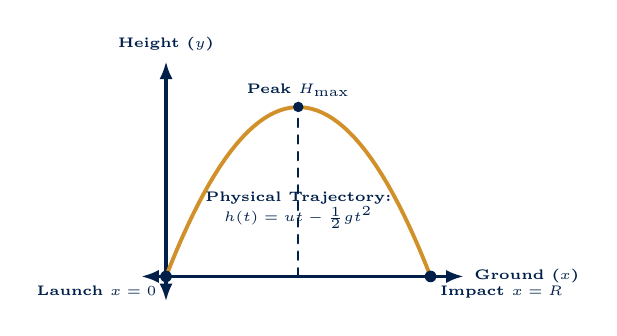
\begin{tikzpicture}[scale=1.05, line cap=round, line join=round]
  % Projectile trajectory
  \draw[{Latex[scale=0.8]}-{Latex[scale=0.8]}, primary, line width=1.1pt] (-0.3,0) -- (3.6,0) node[right, font=\tiny\bfseries]{Ground ($x$)};
  \draw[{Latex[scale=0.8]}-{Latex[scale=0.8]}, primary, line width=1.1pt] (0,-0.3) -- (0,2.6) node[above, font=\tiny\bfseries]{Height ($y$)};

  % Parabola flight path
  \draw[accent, line width=1.4pt, domain=0:3.2, samples=50] plot (\x, {-0.8*\x*(\x-3.2)});

  % Maximum height
  \draw[dashed, reddeep, line width=0.8pt] (1.6,0) -- (1.6,2.05) node[above, font=\tiny\bfseries\color{reddeep}]{Peak $H_{\max}$};
  \fill[reddeep] (1.6,2.05) circle (1.8pt);

  % Launch and Impact points
  \fill[primary] (0,0) circle (2pt) node[below left, font=\tiny\bfseries]{Launch $x=0$};
  \fill[primary] (3.2,0) circle (2pt) node[below right, font=\tiny\bfseries]{Impact $x=R$};

  \node[font=\tiny\bfseries\color{navy}, align=center] at (1.6,0.8) {Physical Trajectory:\\$h(t) = ut - \frac{1}{2}gt^2$};
\end{tikzpicture}
\end{minipage}

\vspace{0.8mm}
\subhead{1.2 Testing Whether an Algebraic Expression is Quadratic}

\begin{warningBox}
  \textbf{\TrapTag\ Never Judge an Equation Before Full Expansion!}
  An equation cannot be classified by visual inspection alone. You must expand all products, clear denominators, and gather all terms to one side:
  \begin{itemize}
    \item Example A: $(x - 2)^2 + 1 = 2x - 3 \implies x^2 - 4x + 4 + 1 = 2x - 3 \implies \mathbf{x^2 - 6x + 8 = 0}$ (\textbf{Quadratic!})
    \item Example B: $x(x + 1) + 8 = (x + 2)(x - 2) \implies x^2 + x + 8 = x^2 - 4 \implies \mathbf{x + 12 = 0}$ (\textbf{Linear, NOT Quadratic!})
    \item Example C: $x + \frac{1}{x} = x^2 \implies x^2 + 1 = x^3 \implies \mathbf{x^3 - x^2 - 1 = 0}$ (\textbf{Cubic, NOT Quadratic!})
  \end{itemize}
\end{warningBox}

\vspace{0.8mm}
\begin{conceptBox}[title={Worked Archetype 1 $\vert$ Algebraic Simplification \& Standard Form Verification},fonttitle=\bfseries\color{navy}]
  \textbf{Problem:} Check whether the equation $(x + 2)^3 = 2x(x^2 - 1)$ is a quadratic equation. If so, write it in standard form.
  \par\vspace{0.6mm}\noindent
  \textbf{Step 1: Expand LHS using algebraic identity $(a + b)^3 = a^3 + 3a^2 b + 3ab^2 + b^3$:}
  $$\text{LHS} = (x + 2)^3 = x^3 + 3(x^2)(2) + 3(x)(2^2) + 2^3 = x^3 + 6x^2 + 12x + 8$$
  \textbf{Step 2: Expand RHS:} $\text{RHS} = 2x(x^2 - 1) = 2x^3 - 2x$.
  \par\noindent
  \textbf{Step 3: Equate LHS and RHS and transfer all terms to one side:}
  $$x^3 + 6x^2 + 12x + 8 = 2x^3 - 2x \implies 2x^3 - x^3 - 6x^2 - 2x - 12x - 8 = 0$$
  $$\mathbf{x^3 - 6x^2 - 14x - 8 = 0}$$
  \textbf{Conclusion:} Since the highest power of $x$ is $3$ (degree is $3$), this is a \textbf{cubic equation, NOT a quadratic equation}.
\end{conceptBox}

\newpage

% =============================================================================
% PAGE 3: MODULE 2 — PARABOLIC GEOMETRY OF ROOTS
% =============================================================================
\thispagestyle{fancy}
\vspace*{0mm}

\chapterbanner{04}{QUADRATIC EQUATIONS}{Module 2 $\vert$ Parabolic Geometry: Roots, Intercepts \& Symmetry}{\CoreTag}

\subhead{2.1 Geometric Meaning of Roots: $x$-Intercepts of a Parabola}

A real number $\alpha$ is called a \textbf{root} (or solution/zero) of the quadratic equation $ax^2 + bx + c = 0$ if and only if $a\alpha^2 + b\alpha + c = 0$.
\begin{itemize}
  \item Geometrically, the roots are the \textbf{$x$-coordinates of the points where the parabola $y = ax^2 + bx + c$ intersects the horizontal $x$-axis}.
  \item Since a parabola can intersect a line in at most two points, a quadratic equation can have \textbf{at most two real roots}.
\end{itemize}

\begin{minipage}[c]{0.45\textwidth}
\centering
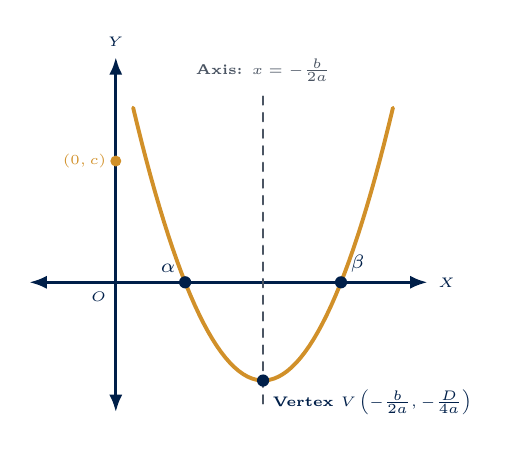
\begin{tikzpicture}[scale=1.1, line cap=round, line join=round]
  % Axes
  \draw[{Latex[scale=0.8]}-{Latex[scale=0.8]}, primary, line width=1.1pt] (-1.0,0) -- (3.6,0) node[right, font=\tiny\bfseries]{$X$};
  \draw[{Latex[scale=0.8]}-{Latex[scale=0.8]}, primary, line width=1.1pt] (0,-1.5) -- (0,2.6) node[above, font=\tiny\bfseries]{$Y$};
  \node[font=\tiny\bfseries\color{navy}, below left] at (0,0) {$O$};

  % Parabola y = (x-0.8)(x-2.6) = x^2 - 3.4x + 2.08
  \draw[accent, line width=1.4pt, domain=0.2:3.2, samples=60] plot (\x, {1.4*(\x-0.8)*(\x-2.6)});

  % Roots alpha and beta
  \fill[reddeep] (0.8,0) circle (2pt) node[above left, font=\scriptsize\bfseries\color{reddeep}]{$\alpha$};
  \fill[reddeep] (2.6,0) circle (2pt) node[above right, font=\scriptsize\bfseries\color{reddeep}]{$\beta$};

  % Axis of symmetry
  \draw[dashed, secondary, line width=0.8pt] (1.7,-1.4) -- (1.7,2.2) node[above, font=\tiny\bfseries]{Axis: $x = -\frac{b}{2a}$};

  % Vertex
  \coordinate (V) at (1.7,-1.134);
  \fill[primary] (V) circle (2pt) node[below right, font=\tiny\bfseries\color{navy}]{Vertex $V\left(-\frac{b}{2a}, -\frac{D}{4a}\right)$};

  % y-intercept (0, c)
  \fill[accent] (0,1.4) circle (1.8pt) node[left, font=\tiny\bfseries\color{accent}]{$(0, c)$};
\end{tikzpicture}
\end{minipage}\hfill
\begin{minipage}[c]{0.53\textwidth}
\begin{formulaBox}
  \textbf{Anatomy of the Quadratic Function $y = ax^2 + bx + c$:}
  \begin{itemize}
    \item \textbf{Curvature Direction:}
      \begin{itemize}
        \item If $a > 0$: Opens upwards ($\cup$, concave up, has a minimum).
        \item If $a < 0$: Opens downwards ($\cap$, concave down, has a maximum).
      \end{itemize}
    \item \textbf{Axis of Symmetry:} Passes through the exact midpoint of roots:
      $$\mathbf{x = \frac{\alpha + \beta}{2} = -\frac{b}{2a}}$$
    \item \textbf{Vertex Coordinates:} Extreme point of parabola:
      $$\mathbf{V\left( -\frac{b}{2a}, \; -\frac{D}{4a} \right)} \quad \text{where } D = b^2 - 4ac$$
    \item \textbf{$y$-Intercept:} Set $x = 0 \implies \mathbf{y = c}$.
  \end{itemize}
\end{formulaBox}
\end{minipage}

\vspace{0.8mm}
\subhead{2.2 The Zero-Product Principle}

\begin{formulaBox}
  \textbf{Fundamental Algebraic Zero-Product Axiom:}
  $$\mathbf{A \cdot B = 0 \iff A = 0 \quad \text{or} \quad B = 0 \quad \text{(or both)}}$$
  If a quadratic equation is factorized into linear factors $(x - \alpha)(x - \beta) = 0$, the roots are $\mathbf{x = \alpha}$ and $\mathbf{x = \beta}$.
\end{formulaBox}

\vspace{0.8mm}
\begin{conceptBox}[title={Worked Archetype 2 $\vert$ Verifying Roots of a Quadratic Equation},fonttitle=\bfseries\color{navy}]
  \textbf{Problem:} Determine whether $x = -1$ and $x = \frac{1}{2}$ are solutions of the equation $2x^2 - x - 1 = 0$.
  \par\vspace{0.6mm}\noindent
  \textbf{Check for $x = -1$:} Substitute $x = -1$ into LHS:
  $$\text{LHS} = 2(-1)^2 - (-1) - 1 = 2(1) + 1 - 1 = 2 \neq 0 \implies \mathbf{x = -1 \text{ is NOT a root.}}$$
  \textbf{Check for $x = 1$:} Substitute $x = 1$ into LHS:
  $$\text{LHS} = 2(1)^2 - (1) - 1 = 2 - 1 - 1 = 0 = \text{RHS} \implies \mathbf{x = 1 \text{ IS a root.}}$$
  \textbf{Check for $x = -\frac{1}{2}$:} $\text{LHS} = 2\left(-\frac{1}{2}\right)^2 - \left(-\frac{1}{2}\right) - 1 = 2\left(\frac{1}{4}\right) + \frac{1}{2} - 1 = \frac{1}{2} + \frac{1}{2} - 1 = 0 \implies \mathbf{x = -\frac{1}{2} \text{ IS a root.}}$
\end{conceptBox}

\newpage

% =============================================================================
% PAGE 4: MODULE 3 — SOLUTION BY FACTORIZATION
% =============================================================================
\thispagestyle{fancy}
\vspace*{0mm}

\chapterbanner{04}{QUADRATIC EQUATIONS}{Module 3 $\vert$ Factoring by Splitting the Middle Term \& Radical Surds}{\CoreTag}

\subhead{3.1 The AC-Method Protocol for Factoring $ax^2 + bx + c = 0$}

To factor $ax^2 + bx + c = 0$, we decompose the middle term $bx$ into two terms $px$ and $qx$ such that:
$$\mathbf{p + q = b} \quad \text{and} \quad \mathbf{p \cdot q = a \cdot c}$$

\begin{minipage}[c]{0.45\textwidth}
\centering
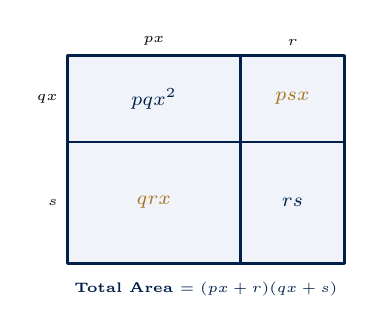
\begin{tikzpicture}[scale=1.1, line cap=round, line join=round]
  % Area model rectangle
  \draw[primary, fill=primarylight, line width=1.2pt] (0,0) rectangle (3.2,2.4);

  % Sub-rectangles
  \draw[primary, line width=0.8pt] (2.0,0) -- (2.0,2.4);
  \draw[primary, line width=0.8pt] (0,1.4) -- (3.2,1.4);

  % Dimensions
  \node[font=\tiny\bfseries, above] at (1.0,2.4) {$px$};
  \node[font=\tiny\bfseries, above] at (2.6,2.4) {$r$};
  \node[font=\tiny\bfseries, left] at (0,1.9) {$qx$};
  \node[font=\tiny\bfseries, left] at (0,0.7) {$s$};

  % Internal areas
  \node[font=\scriptsize\bfseries\color{navy}] at (1.0,1.9) {$pq x^2$};
  \node[font=\scriptsize\bfseries\color{accent!80!black}] at (2.6,1.9) {$ps x$};
  \node[font=\scriptsize\bfseries\color{accent!80!black}] at (1.0,0.7) {$qr x$};
  \node[font=\scriptsize\bfseries\color{navy}] at (2.6,0.7) {$rs$};

  \node[font=\tiny\bfseries\color{navy}, below] at (1.6,-0.1) {Total Area $= (px + r)(qx + s)$};
\end{tikzpicture}
\end{minipage}\hfill
\begin{minipage}[c]{0.53\textwidth}
\begin{formulaBox}
  \textbf{Step-by-Step Factoring Protocol:}
  \begin{enumerate}
    \item Multiply $a$ and $c$ to form the product $P = ac$.
    \item List pairs of factors of $P$ that sum up to $b$.
    \item Split $bx$ as $px + qx$.
    \item Factor by grouping terms in pairs:
      $$ax^2 + px + qx + c = 0$$
    \item Extract common binomial factor:
      $$(px + r)(qx + s) = 0$$
    \item Equate each linear factor to zero to find roots.
  \end{enumerate}
\end{formulaBox}
\end{minipage}

\vspace{0.8mm}
\subhead{3.2 Factoring with Radical (Surd) Coefficients}

\begin{warningBox}
  \textbf{\TrapTag\ Handling Radicals in Middle and Constant Terms:}
  When equations involve square roots like $\sqrt{k}$, calculate $ac$ carefully:
  \begin{itemize}
    \item For $\sqrt{2}x^2 + 7x + 5\sqrt{2} = 0$: Product $ac = (\sqrt{2})(5\sqrt{2}) = 5 \times 2 = \mathbf{10}$.
    \item Find two numbers whose product is $10$ and sum is $7$: $5$ and $2$ ($5 \times 2 = 10, 5 + 2 = 7$).
    \item Rewrite $2x$ strategically as $\sqrt{2} \cdot \sqrt{2}x$ to enable grouping!
  \end{itemize}
\end{warningBox}

\vspace{0.8mm}
\begin{conceptBox}[title={Worked Archetype 3 $\vert$ Factorization with Radical Coefficients},fonttitle=\bfseries\color{navy}]
  \textbf{Problem:} Solve the quadratic equation by factorization: $\sqrt{2}x^2 + 7x + 5\sqrt{2} = 0$.
  \par\vspace{0.6mm}\noindent
  \textbf{Step 1: Compute product $ac$ and target sum $b$:}
  $$a = \sqrt{2}, \quad b = 7, \quad c = 5\sqrt{2} \implies ac = \sqrt{2} \times 5\sqrt{2} = 10$$
  We need factors of $10$ that add up to $7$. The factors are $5$ and $2$.
  \par\noindent
  \textbf{Step 2: Split the middle term $7x$ into $5x + 2x$:}
  $$\sqrt{2}x^2 + 2x + 5x + 5\sqrt{2} = 0$$
  \textbf{Step 3: Group terms in pairs and factor out common elements:}
  Notice that $2 = (\sqrt{2})^2$:
  $$\sqrt{2}x(x + \sqrt{2}) + 5(x + \sqrt{2}) = 0$$
  \textbf{Step 4: Extract common binomial factor $(x + \sqrt{2})$:}
  $$(x + \sqrt{2})(\sqrt{2}x + 5) = 0$$
  \textbf{Step 5: Apply the Zero-Product Principle:}
  $$x + \sqrt{2} = 0 \implies \mathbf{x = -\sqrt{2}} \quad \text{or} \quad \sqrt{2}x + 5 = 0 \implies \mathbf{x = -\frac{5}{\sqrt{2}} = -\frac{5\sqrt{2}}{2}}$$
  \textbf{Final Statement:} The roots of the equation are $\mathbf{-\sqrt{2}}$ and $\mathbf{-\frac{5\sqrt{2}}{2}}$.
\end{conceptBox}

\newpage

% =============================================================================
% PAGE 5: MODULE 4 — THE QUADRATIC FORMULA
% =============================================================================
\thispagestyle{fancy}
\vspace*{0mm}

\chapterbanner{04}{QUADRATIC EQUATIONS}{Module 4 $\vert$ The Quadratic Formula: Sreedharacharya's Classical Derivation}{\CoreTag}

\subhead{4.1 Historical Context: Sreedharacharya's Elegant Technique}

Ancient Indian mathematician \textbf{Sreedharacharya} (c. 8th--9th century CE) derived the universal quadratic formula using a brilliant device: instead of dividing by $a$ (which introduces messy fractions), he \textbf{multiplied the entire equation by $4a$}. This creates an exact square term $(2ax)^2$ and $4abx$, which perfectly completes the binomial square $(2ax + b)^2$!

\begin{center}

\begin{tikzpicture}[scale=0.95, line cap=round, line join=round]
  % Step 1
  \node[draw=primary, fill=primarylight, rounded corners=2mm, line width=1pt, font=\scriptsize\bfseries\color{navy}, align=center, text width=3.8cm] (S1) at (0,2.5) {Standard Form:\\$ax^2 + bx + c = 0$};

  % Step 2
  \node[draw=accent, fill=accentlight, rounded corners=2mm, line width=1pt, font=\scriptsize\bfseries\color{navy}, align=center, text width=4.2cm] (S2) at (5.7,2.5) {Multiply by $4a$ \& shift $c$:\\$4a^2 x^2 + 4abx = -4ac$};

  % Step 3
  \node[draw=primary, fill=primarylight, rounded corners=2mm, line width=1pt, font=\scriptsize\bfseries\color{navy}, align=center, text width=4.5cm] (S3) at (11.4,2.5) {Add $b^2$ to both sides:\\$(2ax + b)^2 = b^2 - 4ac$};

  \draw[-{Stealth[scale=1.1]}, primary, line width=1.3pt] (S1) -- (S2);
  \draw[-{Stealth[scale=1.1]}, accent, line width=1.3pt] (S2) -- (S3);
\end{tikzpicture}
\end{center}

\vspace{0.8mm}
\subhead{4.2 Rigorous Step-by-Step Proof of the Quadratic Formula}

\begin{formulaBox}
  \textbf{Algebraic Derivation of the Formula:}
  \begin{enumerate}
    \item Start with the standard quadratic equation:
      $$ax^2 + bx + c = 0 \quad (a \neq 0)$$
    \item Transpose the constant term to RHS:
      $$ax^2 + bx = -c$$
    \item Multiply the entire equation by $4a$ (Sreedharacharya's device):
      $$4a(ax^2 + bx) = 4a(-c) \implies 4a^2 x^2 + 4abx = -4ac$$
    \item Recognize $4a^2 x^2 = (2ax)^2$ and $4abx = 2(2ax)(b)$. Add $\mathbf{b^2}$ to both sides:
      $$(2ax)^2 + 2(2ax)(b) + b^2 = b^2 - 4ac$$
    \item Factor the LHS as a perfect square:
      $$(2ax + b)^2 = b^2 - 4ac$$
    \item Take the square root of both sides (provided $b^2 - 4ac \ge 0$):
      $$2ax + b = \pm \sqrt{b^2 - 4ac}$$
    \item Solve for $x$ by isolating $2ax$:
      $$2ax = -b \pm \sqrt{b^2 - 4ac} \implies \mathbf{x = \frac{-b \pm \sqrt{b^2 - 4ac}}{2a}}$$
  \end{enumerate}
\end{formulaBox}

\vspace{0.8mm}
\begin{conceptBox}[title={Worked Archetype 4 $\vert$ Application of the Quadratic Formula},fonttitle=\bfseries\color{navy}]
  \textbf{Problem:} Solve the equation $2x^2 - 7x + 3 = 0$ using the quadratic formula.
  \par\vspace{0.6mm}\noindent
  \textbf{Step 1: Identify coefficients:} Comparing with $ax^2 + bx + c = 0 \implies a = 2, \; b = -7, \; c = 3$.\\
  \textbf{Step 2: Calculate the discriminant $D = b^2 - 4ac$:}
  $$D = (-7)^2 - 4(2)(3) = 49 - 24 = \mathbf{25 > 0} \implies \text{Two distinct real roots exist.}$$
  \textbf{Step 3: Substitute into the quadratic formula:}
  $$x = \frac{-(-7) \pm \sqrt{25}}{2(2)} = \frac{7 \pm 5}{4}$$
  \textbf{Step 4: Separate the two roots:}
  $$x_1 = \frac{7 + 5}{4} = \frac{12}{4} = \mathbf{3}, \qquad x_2 = \frac{7 - 5}{4} = \frac{2}{4} = \mathbf{\frac{1}{2}}$$
  \textbf{Conclusion:} The roots are $\mathbf{3}$ and $\mathbf{\frac{1}{2}}$.
\end{conceptBox}

\newpage

% =============================================================================
% PAGE 6: MODULE 5 — THE DISCRIMINANT & NATURE OF ROOTS
% =============================================================================
\thispagestyle{fancy}
\vspace*{0mm}

\chapterbanner{04}{QUADRATIC EQUATIONS}{Module 5 $\vert$ The Discriminant ($D$) \& Tri-State Nature of Roots Matrix}{\CoreTag}

\subhead{5.1 The Discriminant Function $D = b^2 - 4ac$}

In the quadratic formula $x = \frac{-b \pm \sqrt{b^2 - 4ac}}{2a}$, the quantity inside the square root, $\mathbf{D = b^2 - 4ac}$, is called the \textbf{discriminant} because it \textit{discriminates} between the different types of roots.

\begin{center}
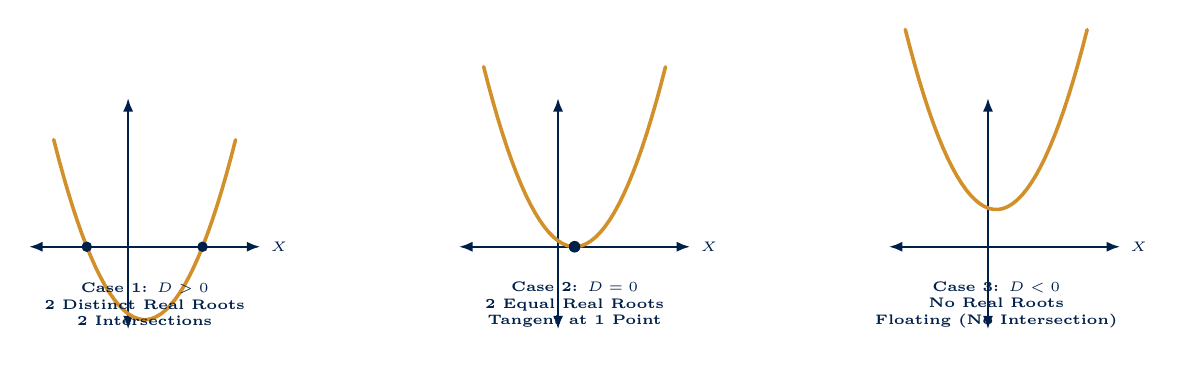
\begin{tikzpicture}[scale=1.05, line cap=round, line join=round]
  % Case 1: D > 0
  \begin{scope}[shift={(0,0)}]
    \draw[{Latex[scale=0.7]}-{Latex[scale=0.7]}, primary, line width=0.9pt] (-1.2,0) -- (1.6,0) node[right, font=\tiny\bfseries]{$X$};
    \draw[{Latex[scale=0.7]}-{Latex[scale=0.7]}, primary, line width=0.9pt] (0,-1.0) -- (0,1.8);
    \draw[accent, line width=1.3pt, domain=-0.9:1.3, samples=40] plot (\x, {1.8*(\x+0.5)*(\x-0.9)});
    \fill[reddeep] (-0.5,0) circle (1.8pt);
    \fill[reddeep] (0.9,0) circle (1.8pt);
    \node[font=\tiny\bfseries\color{navy}, align=center] at (0.2,-0.7) {\textbf{Case 1: $D > 0$}\\2 Distinct Real Roots\\2 Intersections};
  \end{scope}

  % Case 2: D = 0
  \begin{scope}[shift={(5.2,0)}]
    \draw[{Latex[scale=0.7]}-{Latex[scale=0.7]}, primary, line width=0.9pt] (-1.2,0) -- (1.6,0) node[right, font=\tiny\bfseries]{$X$};
    \draw[{Latex[scale=0.7]}-{Latex[scale=0.7]}, primary, line width=0.9pt] (0,-1.0) -- (0,1.8);
    \draw[accent, line width=1.3pt, domain=-0.9:1.3, samples=40] plot (\x, {1.8*(\x-0.2)*(\x-0.2)});
    \fill[reddeep] (0.2,0) circle (2pt);
    \node[font=\tiny\bfseries\color{navy}, align=center] at (0.2,-0.7) {\textbf{Case 2: $D = 0$}\\2 Equal Real Roots\\Tangent at 1 Point};
  \end{scope}

  % Case 3: D < 0
  \begin{scope}[shift={(10.4,0)}]
    \draw[{Latex[scale=0.7]}-{Latex[scale=0.7]}, primary, line width=0.9pt] (-1.2,0) -- (1.6,0) node[right, font=\tiny\bfseries]{$X$};
    \draw[{Latex[scale=0.7]}-{Latex[scale=0.7]}, primary, line width=0.9pt] (0,-1.0) -- (0,1.8);
    \draw[accent, line width=1.3pt, domain=-1.0:1.2, samples=40] plot (\x, {1.8*(\x-0.1)*(\x-0.1) + 0.45});
    \node[font=\tiny\bfseries\color{navy}, align=center] at (0.1,-0.7) {\textbf{Case 3: $D < 0$}\\No Real Roots\\Floating (No Intersection)};
  \end{scope}
\end{tikzpicture}
\end{center}

\vspace{0.8mm}
\subhead{5.2 The Comprehensive Tri-State Nature of Roots Table}

\begin{center}
\small
\begin{tabularx}{\textwidth}{c c p{38mm} X}
\toprule
\rowcolor{bluepale}
\textbf{Condition on $D$} & \textbf{Value of $\sqrt{D}$} & \textbf{Nature of Roots} & \textbf{Exact Formula for Roots} \\
\midrule
$\mathbf{D > 0}$ & Real \& Positive & \textbf{Two distinct real roots} & $x = \frac{-b \pm \sqrt{D}}{2a}$ (Rational if $D$ is perfect square; conjugate surds if not). \\
\rowcolor{lightgray}
$\mathbf{D = 0}$ & Zero ($0$) & \textbf{Two equal real roots} (coincident) & $\mathbf{x = -\frac{b}{2a}, \; -\frac{b}{2a}}$ (Parabola touches $x$-axis at vertex). \\
$\mathbf{D < 0}$ & Imaginary & \textbf{No real roots} & No real values of $x$. Parabola does not touch $x$-axis. \\
\bottomrule
\end{tabularx}
\end{center}

\vspace{0.5mm}
\begin{conceptBox}[title={Worked Archetype 5 $\vert$ Inspecting the Nature of Roots},fonttitle=\bfseries\color{navy}]
  \textbf{Problem:} Find the discriminant of the quadratic equation $2x^2 - 4x + 3 = 0$ and hence find the nature of its roots.
  \par\vspace{0.6mm}\noindent
  \textbf{Solution:} Given $2x^2 - 4x + 3 = 0 \implies a = 2, \; b = -4, \; c = 3$.
  $$D = b^2 - 4ac = (-4)^2 - 4(2)(3) = 16 - 24 = \mathbf{-8}$$
  Since $\mathbf{D < 0}$, the given quadratic equation has \textbf{no real roots}.
\end{conceptBox}

\vspace{0.8mm}
\begin{conceptBox}[title={Worked Archetype 6 $\vert$ Coincident Roots ($D = 0$)},fonttitle=\bfseries\color{navy}]
  \textbf{Problem:} Find the nature of roots of $3x^2 - 2\sqrt{6}x + 2 = 0$. If real roots exist, find them.
  \par\vspace{0.6mm}\noindent
  $$D = b^2 - 4ac = (-2\sqrt{6})^2 - 4(3)(2) = [4 \times 6] - 24 = 24 - 24 = \mathbf{0}$$
  Since $\mathbf{D = 0}$, the equation has \textbf{two equal real roots}:
  $$x = -\frac{b}{2a} = -\frac{-2\sqrt{6}}{2(3)} = \frac{2\sqrt{6}}{6} = \frac{\sqrt{6}}{3} = \mathbf{\sqrt{\frac{2}{3}}}$$
  Hence, both roots are $\mathbf{\sqrt{\frac{2}{3}}}$ and $\mathbf{\sqrt{\frac{2}{3}}}$.
\end{conceptBox}

\newpage

% =============================================================================
% PAGE 7: MODULE 6 — THE PARAMETER k EQUAL-ROOTS PROTOCOL
% =============================================================================
\thispagestyle{fancy}
\vspace*{0mm}

\chapterbanner{04}{QUADRATIC EQUATIONS}{Module 6 $\vert$ The Parameter $k$ Protocol: Condition for Equal Roots ($D = 0$)}{\CoreTag}

\subhead{6.1 The Tangency Condition and Parameter Determination}

A quintessential question in the CBSE Class 10 board examination requires finding the value(s) of an unknown parameter $k$ such that the quadratic equation has \textbf{two equal real roots} (or coincident roots).

\begin{minipage}[c]{0.52\textwidth}
\begin{formulaBox}
  \textbf{The Dual Criteria for Equal Roots:}
  \begin{enumerate}
    \item \textbf{Criterion 1 (Discriminant Zero):}
      $$\mathbf{D = 0 \iff b^2 - 4ac = 0 \iff b^2 = 4ac}$$
    \item \textbf{Criterion 2 (Non-Zero Leading Coefficient):}
      $$\mathbf{a \neq 0}$$
      \textbf{\TrapTag\ The Fatal Parameter Trap:} If the coefficient of $x^2$ contains $k$ (e.g., $a = k - 12$), you \textbf{must explicitly reject} any value of $k$ that makes $a = 0$!
  \end{enumerate}
\end{formulaBox}
\end{minipage}\hfill
\begin{minipage}[c]{0.45\textwidth}
\centering
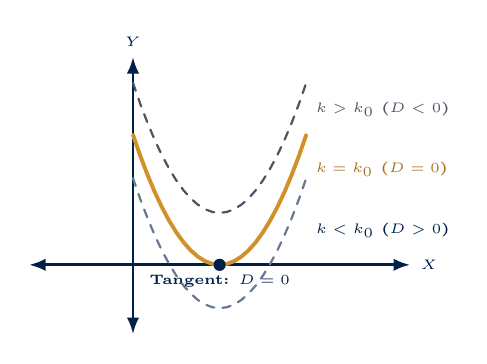
\begin{tikzpicture}[scale=1.1, line cap=round, line join=round]
  % Axes
  \draw[{Latex[scale=0.8]}-{Latex[scale=0.8]}, primary, line width=1pt] (-1.2,0) -- (3.2,0) node[right, font=\tiny\bfseries]{$X$};
  \draw[{Latex[scale=0.8]}-{Latex[scale=0.8]}, primary, line width=1pt] (0,-0.8) -- (0,2.4) node[above, font=\tiny\bfseries]{$Y$};

  % Floating curve (D < 0)
  \draw[dashed, secondary, line width=0.8pt, domain=0:2] plot (\x, {1.5*(\x-1)*(\x-1) + 0.6});
  \node[font=\tiny\bfseries\color{secondary}, right] at (2,1.8) {$k > k_0$ ($D < 0$)};

  % Tangent curve (D = 0)
  \draw[accent, line width=1.4pt, domain=0:2] plot (\x, {1.5*(\x-1)*(\x-1)});
  \fill[reddeep] (1,0) circle (2pt) node[below, font=\tiny\bfseries\color{reddeep}]{Tangent: $D = 0$};
  \node[font=\tiny\bfseries\color{accent!80!black}, right] at (2,1.1) {$k = k_0$ ($D = 0$)};

  % Crossing curve (D > 0)
  \draw[dashed, primary!60, line width=0.8pt, domain=0:2] plot (\x, {1.5*(\x-1)*(\x-1) - 0.5});
  \node[font=\tiny\bfseries\color{primary}, right] at (2,0.4) {$k < k_0$ ($D > 0$)};
\end{tikzpicture}
\end{minipage}

\vspace{0.8mm}
\subhead{6.2 Step-by-Step Equal Roots Solution Protocol}

\begin{enumerate}
  \item Expand all brackets and collect like terms to arrange the equation in strict standard form: $A x^2 + B x + C = 0$.
  \item Write down the expressions for coefficients $a, b, c$ in terms of $k$.
  \item Set up the discriminant equation: $D = b^2 - 4ac = 0$.
  \item Solve the resulting algebraic equation for $k$.
  \item \textbf{Mandatory Check:} Ensure that the values of $k$ do not cause the leading coefficient $a$ to become zero.
\end{enumerate}

\vspace{0.8mm}
\begin{conceptBox}[title={Worked Archetype 7 $\vert$ The Classic Leading Coefficient Trap},fonttitle=\bfseries\color{navy}]
  \textbf{Problem:} Find the value(s) of $k$ for which the quadratic equation $(k - 12)x^2 + 2(k - 12)x + 2 = 0$ has two equal real roots.
  \par\vspace{0.6mm}\noindent
  \textbf{Step 1: Identify coefficients:}
  $$a = k - 12, \quad b = 2(k - 12), \quad c = 2$$
  \textbf{Constraint:} For the equation to remain quadratic, $a \neq 0 \implies k - 12 \neq 0 \implies \mathbf{k \neq 12}$.
  \par\noindent
  \textbf{Step 2: Apply the equal roots condition $D = 0$:}
  $$D = b^2 - 4ac = [2(k - 12)]^2 - 4(k - 12)(2) = 0$$
  $$4(k - 12)^2 - 8(k - 12) = 0$$
  \textbf{Step 3: Factor out the common term $4(k - 12)$ (DO NOT divide by $k-12$ blindly!):}
  $$4(k - 12)\big[ (k - 12) - 2 \big] = 0$$
  $$4(k - 12)(k - 14) = 0$$
  This yields two algebraic solutions:
  $$k - 12 = 0 \implies k = 12 \quad \text{or} \quad k - 14 = 0 \implies k = 14$$
  \textbf{Step 4: Check domain validity:}
  If $k = 12$, then $a = 12 - 12 = 0$, so the equation collapses to $0 \cdot x^2 + 0 \cdot x + 2 = 0 \iff 2 = 0$ (impossible!).\\
  Hence, $\mathbf{k = 12}$ is \textbf{extraneous and must be rejected}.\\
  \textbf{Conclusion:} The only valid value of $k$ is $\mathbf{k = 14}$.
\end{conceptBox}

\newpage

% =============================================================================
% PAGE 8: MODULE 7 — WORD PROBLEMS I: NUMBERS, RECIPROCALS & AGES
% =============================================================================
\thispagestyle{fancy}
\vspace*{0mm}

\chapterbanner{04}{QUADRATIC EQUATIONS}{Module 7 $\vert$ Word Problems I: Numbers, Reciprocals \& Age Models}{\CoreTag}

\subhead{7.1 Translation Protocol from Natural Language to Quadratic Equations}

Word problems test your ability to translate verbal relationships into standard quadratic equations:

\begin{center}
\small
\begin{tabularx}{\textwidth}{p{38mm} p{40mm} X}
\toprule
\rowcolor{bluepale}
\textbf{Verbal Problem Model} & \textbf{Algebraic Representation} & \textbf{Standard Form Equation} \\
\midrule
Two consecutive integers & $x$ and $x + 1$ & Product $= P \implies x(x + 1) = P \implies x^2 + x - P = 0$ \\
\rowcolor{lightgray}
Two consecutive odd/even integers & $x$ and $x + 2$ & Sum of squares $= S \implies x^2 + (x + 2)^2 = S$ \\
A number and its reciprocal & $x$ and $\frac{1}{x}$ ($x \neq 0$) & $x + \frac{1}{x} = \frac{p}{q} \implies qx^2 - px + q = 0$ \\
\rowcolor{lightgray}
Two numbers with sum $S$, product $P$ & $x$ and $S - x$ & $x(S - x) = P \implies x^2 - Sx + P = 0$ \\
Age problems (years ago / hence) & Present age $= x$; Past $= x - n$; Future $= x + m$ & Product of ages $= P \implies (x - n)(x + m) = P$ \\
\bottomrule
\end{tabularx}
\end{center}

\vspace{0.5mm}
\subhead{7.2 Domain Validation: Rejecting Non-Physical Solutions}

\begin{warningBox}
  \textbf{\TrapTag\ Physical Variables Have Strict Domain Restrictions:}
  Quadratic equations mathematically yield two roots. In word problems, you must test both roots against physical reality:
  \begin{itemize}
    \item \textbf{Ages:} Must be positive real numbers ($x > 0$). Reject negative roots!
    \item \textbf{Natural Numbers / Counts:} Must be positive integers ($x \in \mathbb{N}$).
    \item \textbf{Dimensions (Length, Width):} Must be strictly positive ($x > 0$).
  \end{itemize}
\end{warningBox}

\vspace{0.5mm}
\begin{conceptBox}[title={Worked Archetype 8 $\vert$ The Reciprocal Age Problem},fonttitle=\bfseries\color{navy}]
  \textbf{Problem:} The sum of the reciprocals of Rehman's ages (in years) $3\text{ years ago}$ and $5\text{ years from now}$ is $\frac{1}{3}$. Find his present age.
  \par\vspace{0.6mm}\noindent
  \textbf{Step 1: Define the variable:} Let Rehman's present age be $x\text{ years}$ ($x > 3$).\\
  Rehman's age $3\text{ years ago} = (x - 3)\text{ years}$.\\
  Rehman's age $5\text{ years from now} = (x + 5)\text{ years}$.
  \par\noindent
  \textbf{Step 2: Formulate the equation according to given conditions:}
  $$\frac{1}{x - 3} + \frac{1}{x + 5} = \frac{1}{3}$$
  \textbf{Step 3: Combine fractions by taking LCM on LHS:}
  $$\frac{(x + 5) + (x - 3)}{(x - 3)(x + 5)} = \frac{1}{3} \implies \frac{2x + 2}{x^2 + 2x - 15} = \frac{1}{3}$$
  \textbf{Step 4: Cross-multiply and simplify to standard form:}
  $$3(2x + 2) = x^2 + 2x - 15 \implies 6x + 6 = x^2 + 2x - 15$$
  $$x^2 + 2x - 6x - 15 - 6 = 0 \implies \mathbf{x^2 - 4x - 21 = 0}$$
  \textbf{Step 5: Factor by splitting the middle term ($ac = -21, b = -4 \implies -7 \text{ and } 3$):}
  $$(x - 7)(x + 3) = 0 \implies x = 7 \quad \text{or} \quad x = -3$$
  \textbf{Step 6: Physical validation:} Age cannot be negative, so $x = -3$ is rejected.\\
  \textbf{Conclusion:} Rehman's present age is $\mathbf{7\text{ years}}$.
\end{conceptBox}

\newpage

% =============================================================================
% PAGE 9: MODULE 8 — WORD PROBLEMS II: SPEED, DISTANCE & STREAMS
% =============================================================================
\thispagestyle{fancy}
\vspace*{0mm}

\chapterbanner{04}{QUADRATIC EQUATIONS}{Module 8 $\vert$ Word Problems II: Speed, Distance \& River Kinematics}{\CoreTag}

\subhead{8.1 The Speed-Distance-Time Identity: $t = \frac{d}{s}$}

All uniform motion problems rely on the relation $\text{Time} = \frac{\text{Distance}}{\text{Speed}}$.
When speed changes, a time differential $\Delta t$ is created between the slow and fast trips:
$$\mathbf{t_{\text{slow}} - t_{\text{fast}} = \Delta t \implies \frac{d}{s} - \frac{d}{s + v} = \Delta t}$$

\vspace{0.8mm}
\subhead{8.2 River Stream Kinematics (Upstream vs. Downstream)}

\begin{minipage}[c]{0.45\textwidth}
\centering
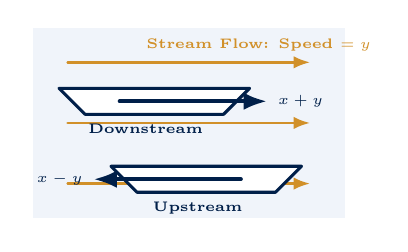
\begin{tikzpicture}[scale=1.1, line cap=round, line join=round]
  % Water stream
  \fill[primarylight] (-0.2,0) rectangle (3.4,2.2);

  % Water flow arrows (to the right)
  \foreach \y in {0.4, 1.1, 1.8} {
    \draw[-{Latex[scale=0.8]}, accent, line width=1pt] (0.2,\y) -- (3.0,\y);
  }
  \node[font=\tiny\bfseries\color{accent}, right] at (1.0,2.0) {Stream Flow: Speed $= y$};

  % Downstream boat
  \draw[primary, fill=white, line width=1.1pt] (0.4,1.2) -- (2.0,1.2) -- (2.3,1.5) -- (0.1,1.5) -- cycle;
  \draw[-{Latex[scale=0.9]}, green, line width=1.4pt] (0.8,1.35) -- (2.5,1.35) node[right, font=\tiny\bfseries\color{green}]{$x + y$};
  \node[font=\tiny\bfseries\color{navy}, below] at (1.1,1.2) {Downstream};

  % Upstream boat
  \draw[primary, fill=white, line width=1.1pt] (1.0,0.3) -- (2.6,0.3) -- (2.9,0.6) -- (0.7,0.6) -- cycle;
  \draw[-{Latex[scale=0.9]}, reddeep, line width=1.4pt] (2.2,0.45) -- (0.5,0.45) node[left, font=\tiny\bfseries\color{reddeep}]{$x - y$};
  \node[font=\tiny\bfseries\color{navy}, below] at (1.7,0.3) {Upstream};
\end{tikzpicture}
\end{minipage}\hfill
\begin{minipage}[c]{0.53\textwidth}
\begin{formulaBox}
  \textbf{Relative Velocities on Water:}
  Let boat speed in still water be $x\text{ km/h}$, and stream speed be $y\text{ km/h}$ ($x > y$):
  \begin{itemize}
    \item \textbf{Downstream (with flow):}
      $$\mathbf{v_{\text{down}} = x + y}$$
    \item \textbf{Upstream (against flow):}
      $$\mathbf{v_{\text{up}} = x - y}$$
    \item \textbf{Time Equation for Distance $d$:}
      Since $x - y < x + y$, upstream travel takes \textbf{longer}:
      $$\mathbf{t_{\text{up}} - t_{\text{down}} = \Delta t \iff \frac{d}{x - y} - \frac{d}{x + y} = \Delta t}$$
  \end{itemize}
\end{formulaBox}
\end{minipage}

\vspace{0.8mm}
\begin{conceptBox}[title={Worked Archetype 9 $\vert$ The Motorboat Stream Problem},fonttitle=\bfseries\color{navy}]
  \textbf{Problem:} A motorboat whose speed is $18\text{ km/h}$ in still water takes $1\text{ hour}$ more to go $24\text{ km}$ upstream than to return downstream to the same spot. Find the speed of the stream.
  \par\vspace{0.6mm}\noindent
  \textbf{Step 1: Set up variables:} Let the speed of the stream be $y\text{ km/h}$ ($0 < y < 18$).\\
  Speed upstream $= (18 - y)\text{ km/h}$, \quad Speed downstream $= (18 + y)\text{ km/h}$.
  \par\noindent
  \textbf{Step 2: Formulate the time equation ($t_{\text{up}} - t_{\text{down}} = 1\text{ hour}$):}
  $$\frac{24}{18 - y} - \frac{24}{18 + y} = 1$$
  \textbf{Step 3: Factor out 24 and combine fractions:}
  $$24\left[ \frac{(18 + y) - (18 - y)}{(18 - y)(18 + y)} \right] = 1 \implies 24\left[ \frac{2y}{324 - y^2} \right] = 1$$
  $$\frac{48y}{324 - y^2} = 1 \implies 48y = 324 - y^2 \implies \mathbf{y^2 + 48y - 324 = 0}$$
  \textbf{Step 4: Factor the quadratic equation ($ac = -324, b = 48 \implies 54 \text{ and } -6$):}
  $$(y + 54)(y - 6) = 0 \implies y = -54 \quad \text{or} \quad y = 6$$
  \textbf{Step 5: Physical validation:} Speed cannot be negative $\implies y = -54$ is rejected.\\
  \textbf{Conclusion:} The speed of the stream is $\mathbf{6\text{ km/h}}$.
\end{conceptBox}

\newpage

% =============================================================================
% PAGE 10: MODULE 9 — WORD PROBLEMS III: WATER TAPS & WORK RATES
% =============================================================================
\thispagestyle{fancy}
\vspace*{0mm}

\chapterbanner{04}{QUADRATIC EQUATIONS}{Module 9 $\vert$ Word Problems III: Water Taps, Cisterns \& Unit Work Rates}{\CoreTag}

\subhead{10.1 The Unit Work Rate Principle}

If a pipe or worker can complete a task in $T\text{ hours}$, then in $1\text{ hour}$, the fraction of work completed is exactly $\mathbf{\frac{1}{T}}$.
When two pipes work simultaneously, their individual flow rates add up to equal the combined flow rate:

\begin{minipage}[c]{0.45\textwidth}
\centering
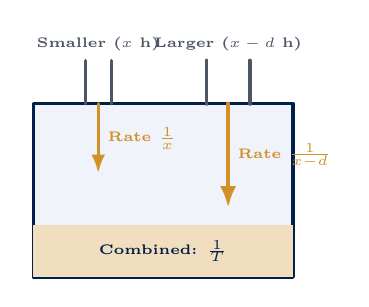
\begin{tikzpicture}[scale=1.1, line cap=round, line join=round]
  % Cistern / Tank
  \draw[primary, fill=primarylight, line width=1.2pt] (0,0) rectangle (3.0,2.0);

  % Tap 1 (Smaller)
  \draw[secondary, line width=1.1pt] (0.6,2.5) -- (0.6,2.0);
  \draw[secondary, line width=1.1pt] (0.9,2.5) -- (0.9,2.0);
  \draw[-{Latex[scale=0.8]}, accent, line width=1.2pt] (0.75,2.0) -- (0.75,1.2);
  \node[font=\tiny\bfseries\color{secondary}, above] at (0.75,2.5) {Smaller ($x\text{ h}$)};
  \node[font=\tiny\bfseries\color{accent}, right] at (0.75,1.6) {Rate $\frac{1}{x}$};

  % Tap 2 (Larger)
  \draw[secondary, line width=1.4pt] (2.0,2.5) -- (2.0,2.0);
  \draw[secondary, line width=1.4pt] (2.5,2.5) -- (2.5,2.0);
  \draw[-{Latex[scale=0.8]}, accent, line width=1.5pt] (2.25,2.0) -- (2.25,0.8);
  \node[font=\tiny\bfseries\color{secondary}, above] at (2.25,2.5) {Larger ($x - d\text{ h}$)};
  \node[font=\tiny\bfseries\color{accent}, right] at (2.25,1.4) {Rate $\frac{1}{x - d}$};

  % Water level
  \fill[accent!30] (0,0) rectangle (3.0,0.6);
  \node[font=\tiny\bfseries\color{navy}] at (1.5,0.3) {Combined: $\frac{1}{T}$};
\end{tikzpicture}
\end{minipage}\hfill
\begin{minipage}[c]{0.53\textwidth}
\begin{formulaBox}
  \textbf{Master Tap Flow Rate Equation:}
  Let smaller tap take $x\text{ hours}$, and larger tap take $(x - d)\text{ hours}$ to fill tank alone:
  $$\mathbf{\text{Rate of Tap 1} = \frac{1}{x}}$$
  $$\mathbf{\text{Rate of Tap 2} = \frac{1}{x - d}}$$
  $$\mathbf{\text{Combined Rate} = \frac{1}{x} + \frac{1}{x - d} = \frac{1}{T_{\text{together}}}}$$
  \textit{Clearing denominators produces a clean quadratic equation in $x$!}
\end{formulaBox}
\end{minipage}

\vspace{0.8mm}
\begin{conceptBox}[title={Worked Archetype 10 $\vert$ Two Water Taps Filling a Tank Together},fonttitle=\bfseries\color{navy}]
  \textbf{Problem:} Two water taps together can fill a tank in $9\frac{3}{8}\text{ hours}$ ($=\frac{75}{8}\text{ hours}$). The tap of larger diameter takes $10\text{ hours}$ less than the smaller one to fill the tank separately. Find the time in which each tap can separately fill the tank.
  \par\vspace{0.6mm}\noindent
  \textbf{Step 1: Define variables:}
  Let time taken by smaller tap alone $= x\text{ hours}$ ($x > 10$).\\
  Time taken by larger tap alone $= (x - 10)\text{ hours}$.\\
  Combined time $T = \frac{75}{8}\text{ hours} \implies \text{Combined 1-hour rate} = \frac{1}{T} = \frac{8}{75}$.
  \par\noindent
  \textbf{Step 2: Set up the flow rate equation:}
  $$\frac{1}{x} + \frac{1}{x - 10} = \frac{8}{75}$$
  \textbf{Step 3: Combine LHS and cross-multiply:}
  $$\frac{(x - 10) + x}{x(x - 10)} = \frac{8}{75} \implies \frac{2x - 10}{x^2 - 10x} = \frac{8}{75}$$
  Divide numerator of LHS and RHS by $2$:
  $$\frac{x - 5}{x^2 - 10x} = \frac{4}{75} \implies 75(x - 5) = 4(x^2 - 10x)$$
  $$75x - 375 = 4x^2 - 40x \implies \mathbf{4x^2 - 115x + 375 = 0}$$
  \textbf{Step 4: Solve the quadratic equation by factoring ($ac = 4 \times 375 = 1500, b = -115 \implies -100 \text{ and } -15$):}
  $$4x^2 - 100x - 15x + 375 = 0 \implies 4x(x - 25) - 15(x - 25) = 0$$
  $$(x - 25)(4x - 15) = 0 \implies x = 25 \quad \text{or} \quad x = \frac{15}{4} = 3.75$$
  \textbf{Step 5: Physical validity check:}
  If $x = 3.75\text{ hours}$, then time for larger tap $= 3.75 - 10 = -6.25\text{ hours}$ (impossible!).\\
  Hence, $x = 3.75$ is \textbf{rejected}, and we accept $\mathbf{x = 25}$.\\
  \textbf{Conclusion:} Time for smaller tap alone is $\mathbf{25\text{ hours}}$, and for larger tap alone is $\mathbf{15\text{ hours}}$.
\end{conceptBox}

\newpage

% =============================================================================
% PAGE 11: MODULE 10 — WORD PROBLEMS IV: GEOMETRY & PATHWAYS
% =============================================================================
\thispagestyle{fancy}
\vspace*{0mm}

\chapterbanner{04}{QUADRATIC EQUATIONS}{Module 10 $\vert$ Word Problems IV: Geometry, Mensuration \& Pathways}{\CoreTag}

\subhead{11.1 Geometric Formulations via Pythagoras \& Area Theorems}

Mensuration word problems translate spatial configurations into quadratic forms:
\begin{itemize}
  \item \textbf{Right Triangles:} Hypotenuse $c$, sides $x$ and $x - d \implies \mathbf{x^2 + (x - d)^2 = c^2}$.
  \item \textbf{Rectangular Fields with Uniform Borders:} An inner lawn $(l \times b)$ surrounded by a path of width $w$:
    $$\text{Outer Length} = l + 2w, \quad \text{Outer Breadth} = b + 2w \implies \mathbf{\text{Area of Path} = (l + 2w)(b + 2w) - lb}$$
\end{itemize}

\begin{minipage}[c]{0.45\textwidth}
\centering
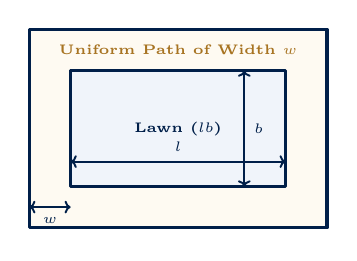
\begin{tikzpicture}[scale=1.05, line cap=round, line join=round]
  % Outer boundary
  \draw[primary, fill=accentlight, line width=1.2pt] (-1.8,-1.2) rectangle (1.8,1.2);
  % Inner lawn
  \draw[primary, fill=primarylight, line width=1.1pt] (-1.3,-0.7) rectangle (1.3,0.7);

  % Dimension arrows
  \draw[{<[scale=0.7]}-{>[scale=0.7]}, primary, line width=0.7pt] (-1.3,-0.4) -- (1.3,-0.4) node[midway, above, font=\tiny\bfseries]{$l$};
  \draw[{<[scale=0.7]}-{>[scale=0.7]}, primary, line width=0.7pt] (0.8,-0.7) -- (0.8,0.7) node[midway, right, font=\tiny\bfseries]{$b$};

  \draw[{<[scale=0.7]}-{>[scale=0.7]}, reddeep, line width=0.7pt] (-1.8,-0.95) -- (-1.3,-0.95) node[midway, below, font=\tiny\bfseries\color{reddeep}]{$w$};

  \node[font=\tiny\bfseries\color{navy}] at (0,0) {Lawn ($lb$)};
  \node[font=\tiny\bfseries\color{accent!80!black}] at (0,0.95) {Uniform Path of Width $w$};
\end{tikzpicture}
\end{minipage}\hfill
\begin{minipage}[c]{0.53\textwidth}
\centering
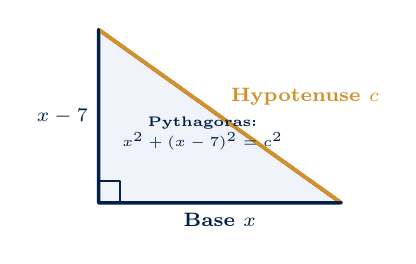
\begin{tikzpicture}[scale=1.1, line cap=round, line join=round]
  % Right triangle
  \coordinate (A) at (0,2.0);
  \coordinate (B) at (0,0);
  \coordinate (C) at (2.8,0);

  \draw[primary, fill=primarylight, line width=1.2pt] (A) -- (B) -- (C) -- cycle;
  \draw[accent, line width=1.4pt] (A) -- (C) node[midway, above right, font=\scriptsize\bfseries\color{accent}]{Hypotenuse $c$};

  % Sides
  \draw[primary, line width=1.1pt] (A) -- (B) node[midway, left, font=\scriptsize\bfseries]{$x - 7$};
  \draw[primary, line width=1.1pt] (B) -- (C) node[midway, below, font=\scriptsize\bfseries]{Base $x$};

  % Right angle mark
  \draw[reddeep, line width=0.7pt] (0,0.25) -- (0.25,0.25) -- (0.25,0);
  \node[font=\tiny\bfseries\color{navy}, align=center] at (1.2,0.8) {Pythagoras:\\$x^2 + (x - 7)^2 = c^2$};
\end{tikzpicture}
\end{minipage}

\vspace{0.8mm}
\begin{conceptBox}[title={Worked Archetype 11 $\vert$ Right Triangle Altitude and Base Relationship},fonttitle=\bfseries\color{navy}]
  \textbf{Problem:} The altitude of a right triangle is $7\text{ cm}$ less than its base. If the hypotenuse is $13\text{ cm}$, find the other two sides.
  \par\vspace{0.6mm}\noindent
  \textbf{Step 1: Formulate variables:} Let base $= x\text{ cm}$ ($x > 7$). Altitude $= (x - 7)\text{ cm}$. Hypotenuse $= 13\text{ cm}$.\\
  \textbf{Step 2: Apply Pythagoras Theorem:}
  $$\text{Base}^2 + \text{Altitude}^2 = \text{Hypotenuse}^2 \implies x^2 + (x - 7)^2 = 13^2$$
  \textbf{Step 3: Expand and simplify to standard form:}
  $$x^2 + (x^2 - 14x + 49) = 169 \implies 2x^2 - 14x + 49 - 169 = 0$$
  $$2x^2 - 14x - 120 = 0 \implies \text{Divide by 2: } \mathbf{x^2 - 7x - 60 = 0}$$
  \textbf{Step 4: Factor the quadratic equation ($ac = -60, b = -7 \implies -12 \text{ and } 5$):}
  $$(x - 12)(x + 5) = 0 \implies x = 12 \quad \text{or} \quad x = -5$$
  \textbf{Step 5: Physical validation:} Side length cannot be negative $\implies x = -5$ is rejected.\\
  $$\text{Base } x = \mathbf{12\text{ cm}}, \quad \text{Altitude } = x - 7 = 12 - 7 = \mathbf{5\text{ cm}}$$
  \textbf{Verification:} $12^2 + 5^2 = 144 + 25 = 169 = 13^2$ (Pythagorean triplet verified!).
\end{conceptBox}

\newpage

% =============================================================================
% PAGE 12: MODULE 11 — MASTER FORMULA MATRIX & DECISION TREE
% =============================================================================
\thispagestyle{fancy}
\vspace*{0mm}

\chapterbanner{04}{QUADRATIC EQUATIONS}{Module 11 $\vert$ Master Formula Matrix \& Solution Decision Protocol}{\ReferenceTag}

\subhead{11.1 The Comprehensive Quadratic Equations Matrix}

\begin{center}
\small
\begin{tabularx}{\textwidth}{>{\bfseries}p{32mm} c p{38mm} X}
\toprule
\rowcolor{bluepale}
Method / Theorem & Prerequisite Form & Mathematical Rule & Strategic Board Examination Purpose \\
\midrule
Standard Form & $a \neq 0$ & $ax^2 + bx + c = 0$ & Mandatory first step for all quadratic methods. \\
\rowcolor{lightgray}
Factorization & $p \cdot q = ac, \; p+q = b$ & $(px + r)(qx + s) = 0$ & Fastest method when $ac$ factors cleanly. \\
Quadratic Formula & $D \ge 0$ & $x = \frac{-b \pm \sqrt{b^2 - 4ac}}{2a}$ & Universal method; handles surd/radical coefficients. \\
\rowcolor{lightgray}
Discriminant $D$ & $D = b^2 - 4ac$ & $D > 0, \; D = 0, \; D < 0$ & Testing nature of roots without solving equation. \\
Equal Roots Condition & Two equal roots & $b^2 - 4ac = 0$ with $a \neq 0$ & Finding unknown parameter $k$ (high frequency!). \\
\rowcolor{lightgray}
Parabola Vertex & Axis of symmetry & $x = -\frac{b}{2a}, \; y = -\frac{D}{4a}$ & Extreme values / trajectory height peak. \\
Sum \& Product & Roots $\alpha, \beta$ & $\alpha + \beta = -\frac{b}{a}, \; \alpha\beta = \frac{c}{a}$ & Fast verification check of computed roots. \\
\bottomrule
\end{tabularx}
\end{center}

\vspace{0.8mm}
\subhead{11.2 The 3-Tier Board Problem Decision Flowchart}

\begin{center}

\begin{tikzpicture}[scale=0.95, line cap=round, line join=round]
  % Step 1
  \node[draw=primary, fill=primarylight, rounded corners=2mm, line width=1pt, font=\scriptsize\bfseries\color{navy}, align=center, text width=4.5cm] (Q1) at (0,2.5) {TIER 1: Standard Form\\Arrange as $ax^2 + bx + c = 0$\\Check $a \neq 0$};

  % Step 2
  \node[draw=accent, fill=accentlight, rounded corners=2mm, line width=1pt, font=\scriptsize\bfseries\color{navy}, align=center, text width=4.5cm] (Q2) at (5.7,2.5) {TIER 2: Compute $D = b^2 - 4ac$\\Is $D > 0$, $D = 0$, or $D < 0$?\\($D < 0 \implies \text{Stop: No Real Roots}$)};

  % Step 3
  \node[draw=primary, fill=primarylight, rounded corners=2mm, line width=1pt, font=\scriptsize\bfseries\color{navy}, align=center, text width=4.5cm] (Q3) at (11.4,2.5) {TIER 3: Choose Method\\Is $D$ a perfect square?\\Yes $\implies$ Factor; No $\implies$ Formula};

  \draw[-{Stealth[scale=1.1]}, primary, line width=1.3pt] (Q1) -- (Q2);
  \draw[-{Stealth[scale=1.1]}, accent, line width=1.3pt] (Q2) -- (Q3);
\end{tikzpicture}
\end{center}

\vspace{0.8mm}
\begin{formulaBox}
  \textbf{Fast Mental-Math Factoring Rules:}
  \begin{itemize}
    \item \textbf{Sign of $c$ is Positive ($c > 0$):} Both factors must have the \textbf{same sign} (the sign of $b$).
      \begin{itemize}
        \item $x^2 - 8x + 12 = 0 \implies b < 0, c > 0 \implies$ both negative: $(x - 6)(x - 2) = 0$.
        \item $x^2 + 8x + 12 = 0 \implies b > 0, c > 0 \implies$ both positive: $(x + 6)(x + 2) = 0$.
      \end{itemize}
    \item \textbf{Sign of $c$ is Negative ($c < 0$):} Factors have \textbf{opposite signs}; the larger factor takes the sign of $b$.
      \begin{itemize}
        \item $x^2 - x - 12 = 0 \implies b < 0, c < 0 \implies$ larger factor is negative: $(x - 4)(x + 3) = 0$.
      \end{itemize}
  \end{itemize}
\end{formulaBox}

\newpage

% =============================================================================
% PAGE 13: MODULE 12 — BOARD EXAM CASE-STUDY & CONTEXTUAL MODELING
% =============================================================================
\thispagestyle{fancy}
\vspace*{0mm}

\chapterbanner{04}{QUADRATIC EQUATIONS}{Module 12 $\vert$ Applied Case-Study: Projectile Motion \& Parabolic Flight}{\ExamTag}

\subhead{Case Study 1 $\vert$ Fire Service Water Cannon Trajectory}

A specialized fire-fighting truck sprays water through a pressurized cannon. The height $h$ (in meters) of the water jet above the ground at a horizontal distance $x$ (in meters) from the nozzle is modeled by the quadratic equation:
$$h(x) = -\frac{1}{20}x^2 + x + 1.25$$

\begin{minipage}[c]{0.42\textwidth}
\centering
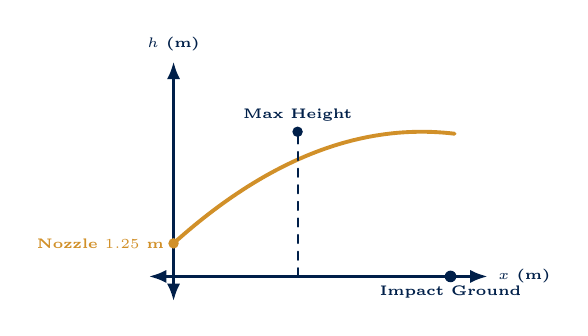
\begin{tikzpicture}[scale=1.05, line cap=round, line join=round]
  % Ground
  \draw[{Latex[scale=0.8]}-{Latex[scale=0.8]}, primary, line width=1.1pt] (-0.3,0) -- (3.8,0) node[right, font=\tiny\bfseries]{$x\text{ (m)}$};
  \draw[{Latex[scale=0.8]}-{Latex[scale=0.8]}, primary, line width=1.1pt] (0,-0.3) -- (0,2.6) node[above, font=\tiny\bfseries]{$h\text{ (m)}$};

  % Trajectory h(x) = -0.05 x^2 + x + 1.25. Peak at x = 10, h = 6.25. Zero at x = 21.18
  \draw[accent, line width=1.4pt, domain=0:3.4, samples=50] plot (\x, {-0.15*\x*\x + 0.9*\x + 0.4});

  % Nozzle height
  \fill[accent] (0,0.4) circle (1.8pt) node[left, font=\tiny\bfseries\color{accent}]{Nozzle $1.25\text{ m}$};

  % Peak
  \draw[dashed, reddeep, line width=0.7pt] (1.5,0) -- (1.5,1.75) node[above, font=\tiny\bfseries\color{reddeep}]{Max Height};
  \fill[reddeep] (1.5,1.75) circle (1.8pt);

  % Impact on ground
  \fill[primary] (3.35,0) circle (2pt) node[below, font=\tiny\bfseries]{Impact Ground};
\end{tikzpicture}
\end{minipage}\hfill
\begin{minipage}[c]{0.56\textwidth}
\begin{conceptBox}[title={4-Mark Board Question Protocol},fonttitle=\bfseries\color{navy}]
  \textbf{Questions:}
  \begin{enumerate}
    \item What is the height of the nozzle from the ground? [1M]
    \item At what horizontal distance does the water jet reach its maximum height? [1M]
    \item Find the horizontal distance from the nozzle where the water jet strikes the ground. [2M]
  \end{enumerate}
\end{conceptBox}
\end{minipage}

\vspace{0.8mm}
\begin{successBox}[title={Solution \& Marking Scheme Evaluation},fonttitle=\bfseries\color{navy}]
  \begin{enumerate}
    \item \textbf{Height of Nozzle [1M]:} At the nozzle, the horizontal distance is $x = 0$:
      $$h(0) = -\frac{1}{20}(0)^2 + (0) + 1.25 = \mathbf{1.25\text{ meters}}$$
    \item \textbf{Distance for Maximum Height [1M]:} Maximum height occurs at the vertex $x = -\frac{b}{2a}$:
      $$a = -\frac{1}{20} = -0.05, \quad b = 1 \implies x = -\frac{1}{2(-0.05)} = -\frac{1}{-0.1} = \mathbf{10\text{ meters}}$$
    \item \textbf{Impact Horizontal Distance [2M]:} Water strikes ground when height $h(x) = 0$:
      $$-\frac{1}{20}x^2 + x + 1.25 = 0 \implies \text{Multiply by } -20: \quad \mathbf{x^2 - 20x - 25 = 0}$$
      Apply the quadratic formula with $a = 1, b = -20, c = -25$:
      $$D = (-20)^2 - 4(1)(-25) = 400 + 100 = 500$$
      $$x = \frac{-(-20) \pm \sqrt{500}}{2(1)} = \frac{20 \pm 10\sqrt{5}}{2} = 10 \pm 5\sqrt{5}$$
      Since distance must be positive, take the positive root ($\sqrt{5} \approx 2.236$):
      $$x = 10 + 5(2.236) = 10 + 11.18 = \mathbf{21.18\text{ meters}}$$
  \end{enumerate}
\end{successBox}

\newpage

% =============================================================================
% PAGE 14: MODULE 13 — CBSE BOARD TRAPS, HACKS & PRE-SUBMISSION AUDIT
% =============================================================================
\thispagestyle{fancy}
\vspace*{0mm}

\chapterbanner{04}{QUADRATIC EQUATIONS}{Module 13 $\vert$ Board Traps, Verification Hacks \& 5-Point Audit}{\ExamTag}

\subhead{13.1 The Top 7 Quadratic Equation Board Traps (And How to Bust Them)}

\begin{enumerate}[label=\textbf{Trap \arabic*:}, leftmargin=5mm, itemsep=1pt, topsep=0.8pt, parsep=0pt]
  \item \textbf{The Variable Division Cancellation Trap:} Solving $x^2 = 5x$ by dividing both sides by $x$ to get $x = 5$. \TrapTag\ You lose the valid root $\mathbf{x = 0}$! Always factor: $x^2 - 5x = 0 \implies x(x - 5) = 0 \implies x = 0, 5$.
  \item \textbf{The Negative Linear Coefficient Sign Error:} In $x = \frac{-b \pm \sqrt{D}}{2a}$, when $b = -7$, writing $-7 \pm \dots$ instead of $-(-7) = \mathbf{+7}$.
  \item \textbf{The Squaring Negative $b$ Blunder:} Writing $(-6)^2 = -36$ inside $b^2 - 4ac$. Any real number squared is non-negative: $\mathbf{(-6)^2 = +36}$!
  \item \textbf{The Parameter $a \neq 0$ Violation:} In $(k - 1)x^2 + 2x + 1 = 0$, finding $k = 1$ from $D = 0$ but forgetting that $k = 1$ makes $a = 0$. You \textbf{must reject} values making the leading coefficient zero!
  \item \textbf{Upstream vs. Downstream Subtraction Order:} Writing downstream time minus upstream time as positive. Upstream is always \textbf{slower}, so $\mathbf{t_{\text{upstream}} > t_{\text{downstream}}}$.
  \item \textbf{Retaining Extraneous Negative Roots in Word Problems:} Forgetting to state: "Since speed/age/time cannot be negative, $x = -k$ is rejected."
  \item \textbf{Using the Deleted "Completing the Square" Method:} In CBSE 2026--27, solve strictly using \textbf{Factorization} or the \textbf{Quadratic Formula}.
\end{enumerate}

\subhead{13.2 High-Speed Algebraic Verification Protocol (Vieta's Relations)}

After calculating roots $\alpha$ and $\beta$, check them mentally in 5 seconds using Vieta's formulas:
$$\mathbf{\text{Sum of Roots: } \alpha + \beta = -\frac{b}{a}} \qquad \text{and} \qquad \mathbf{\text{Product of Roots: } \alpha \cdot \beta = \frac{c}{a}}$$
If the sum or product does not match the original equation coefficients, an arithmetic error occurred!

\vspace{1mm}
\subhead{13.3 The 5-Point Board Examination Pre-Submission Checklist}

\begin{successBox}[top=1.2mm,bottom=1.2mm,before skip=1.5pt,after skip=1pt]
  \textbf{Final 60-Second Answer Sheet Verification Protocol:}
  \begin{itemize}[leftmargin=4mm,itemsep=1pt,topsep=1pt,parsep=0pt]
    \item[$\square$] \textbf{Standard Form Established:} Did you gather all terms to one side ($ax^2 + bx + c = 0$) before identifying $a, b, c$?
    \item[$\square$] \textbf{Discriminant Sign Verified:} Did you compute $D = b^2 - 4ac$ accurately with correct sign multiplication ($-4ac$)?
    \item[$\square$] \textbf{Two Roots Recorded:} Did you state both roots explicitly? (Quadratic equations have 2 roots!).
    \item[$\square$] \textbf{Physical Feasibility Justified:} For word problems, did you write an explicit sentence rejecting the negative root?
    \item[$\square$] \textbf{Correct Dimensional Units Attached:} Speeds in $\mathbf{\text{km/h}}$, Times in $\mathbf{\text{hours}}$, Dimensions in $\mathbf{\text{cm} / \text{m}}$!
  \end{itemize}
\end{successBox}

\vfill
\begin{center}
  {\footnotesize\bfseries\color{primary}MATHS MANTHAN TUITION CLASSES \quad$\vert$\quad END OF CHAPTER 4 HANDBOOK}\\[1mm]
  {\scriptsize\color{secondary}Designed for Academic Excellence in CBSE Class 10 Board Examinations 2026--27.}
\end{center}

\end{document}
